\setcounter{chapter}{1}
\chapter{Neuroanatomy}
\label{sec:neuro}
% \minitoc
%
\comment{\paragraph{Ziele:} 
\begin{itemize}
    \item uebersicht neuroanatomy
    \item struktureller aufbau nervenfaser
    \item ableitbare eigenschaften fuer modelle
\end{itemize}}
%
\section{Evolution/Introduction}
%
\section{Brain Architecture}
%
\begin{figure}[!t]
	\centering
% 	\resizebox{0.75\textwidth}{!}{
\subcaptionbox{}[.28\textwidth]{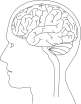
\includegraphics[height=3cm]{gfx/neuroanatomy/human-brain-profile.pdf}}
\subcaptionbox{}[.35\textwidth]{\includegraphics[height=3cm]{gfx/neuroanatomy/human-brain-section.pdf}}
\subcaptionbox{}[.35\textwidth]{\includegraphics[height=3cm]{gfx/neuroanatomy/neuron-axon.pdf}}
% 	}
	\caption{(a) Illustration of human brain. (b) Illustration of a coronal human brain section. (c) Illustration of a neuron with axon and oligodendrocytes.}
	\label{fig::human-brain}
\end{figure}
%
\section{Fiber Architecture}
%
\section{Sectioning}
%
\begin{figure}[!t]
	\centering
    \def\tikzwidth{\textwidth}
	\inputtikz{gfx/neuroanatomy/brain_sectioning.tikz}
	\caption{Illustration of sectioning.}
	\label{fig::brain_sectioning}
\end{figure}
%
\section{Microscopy}
% 
Axon diameter \cite{Liewald2014}:
% 
\begin{table}[!b]
\centering
\pgfplotstabletypeset[
thesis,
col sep=comma,
columns/Name/.style={string type},
columns/Mean/.style={fixed zerofill},
columns/SD/.style={fixed zerofill},
columns/Median/.style={fixed zerofill},
columns/Max/.style={fixed zerofill},
columns/Min/.style={fixed zerofill},
columns/n/.style={dec sep align},
]{data/axon_distribution.csv}
\caption{axon diameter distribution of the human brain in \si{\micro\meter} \cite{Liewald2014}}
\end{table}
axon = 0.5-1.0 diameter (most frequent
thickness of myelin mean = 0.09, median 0.08
-> g-ratio 0.9 (electron microscop, upper boundry)
% 
g-ratio
\cite{Cercignani2017} -> 0.65-0.8 mrt, healty male and female different age, different regions\\
\cite{FitzGibbon2013} -> 0.58-0.84 (Retina), electron microscopy
